\section{Suivi de la main dans une séquence d’images}
\subsection{Présentation de la méthode}

Les images du groupe 2, qui constituent une succession d’images, ne peuvent être traitées de la même manière que celles des deux autres groupes. En effet, notre méthode de segmentation telle qu’elle est conçue est idéale sur des images dans lesquelles la main est en avant-plan, ce qui n’est pas le cas sur l’ensemble d’images de ce groupe.
	Nous avons donc développé une méthode de traitement spéciale pour ce groupe, effectuant un suivi de la main dans l’image. L’idée générale de notre méthode est de suivre la main d’une image à l’autre afin de seuiller et ne garder uniquement la partie de l’image qui contient la main. Un tel algorithme pourrait être utilisé pour réaliser du suivi de main dans une séquence d’images quelconque, indépendamment de la reconnaissance. Notre méthode nécessite cependant de bénéficier à la base d’une image propre sur laquelle il est possible de réaliser une segmentation idéale.
	L’algorithme de suivi de la main est basé sur l’opérateur de Harris. Il permet d’effectuer un seuillage localisé sur la main d’une image à l’autre. Afin de localiser la main, on part à la base d’une image seuillée et on calcule la boîte englobante de la main. Cette même boîte englobante est utilisée sur l’image suivante de sorte que l’on obtienne deux fenêtres d’intérêt pour chaque image, partant du postulat que d’une image à l’autre, le mouvement de la main est minime. L’opérateur de Harris est alors appliqué sur chaque fenêtre (chaque main) de deux images consécutives. Après un appariement des points, on peut calculer un mouvement de la main par distance euclidienne de deux points appariés. Une nouvelle boîte sur laquelle on applique le mouvement est alors calculée et appliquée à la seconde image. Cette méthode est théoriquement efficace pour des mouvements latéraux de la main, mais lorsque celle-ci se rapproche ou s’éloigne de la caméra, un ajustement est nécessaire. C’est la raison pour laquelle la taille d’une boite englobante est élargie avant seuillage puis réadaptée.

L’algorithme développé peut être écrit comme suit :

\begin{itemize}
\item Segmentation de la main sur la première image.
\item Création de la boîte englobante (box).
\item Opérateur de Harris pour identifier les points d’intérêts.
\item Boucle : Pour chaque image consécutive
\begin{itemize}
\item Elargissement de la box.
\item Seuillage à l’intérieur de la box afin d’extraire la main.
\item Recadrage de la box si nécessaire.
\item Opérateur de Harris pour identifier les points d’intérêts.
\item Appariement des points de l’image seuillée et de la précédente.
\item Application du mouvement de la main sur le déplacement de la box.
\end{itemize}
\end{itemize}

\subsubsection{Segmentation de la main et extraction de la box}
Cette segmentation est « banale » et réutilise la méthode de segmentation générale basée sur l’algorithme de Fisher. A partir de l’image binarisée résultante, il est très simple de calculer les coordonnées de la boite englobante de la main extraite (\autoref{fig:boundingBox}).

\begin{figure}[htb!]
\centerline{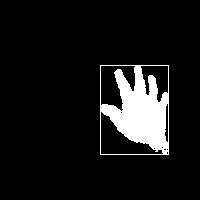
\includegraphics{boundingBox.jpg}}
\caption{Boîte englobante d'une main extraite.}
\label{fig:boundingBox}
\end{figure}

\subsubsection{Opérateur de Harris}
Dans la seconde étape importante, l’opérateur de Harris a été utilisé afin d’extraire les points d’intérêt de l’image seuillée. Ces points d’intérêt auraient pu être calculés sur l’image source, mais d’une image à l’autre, l’expérience a prouvé qu’aucuns points ne correspondaient, ce qui s'avérait problématique pour réaliser l’appariement d’une image à l’autre et détecter un mouvement. Sur l’image suivante, on observe les contours de la main ainsi que les points d’intérêt en blanc (\autoref{fig:harris}).

\begin{figure}[htb!]
\centerline{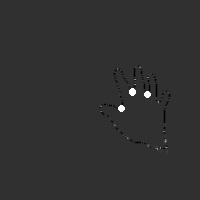
\includegraphics{harris.jpg}}
\caption{Points d'intérêts de la main par l'opérateur de Harris.}
\label{fig:harris}
\end{figure}

Pour chaque image consécutive :

\subsubsection{Seuillage sur la boite englobante}

Afin de préparer le terrain à l’opérateur de Harris, il est nécessaire de seuiller chaque image. L’identification du seuil est l’étape de l’algorithme qui présente le plus de problèmes et également celle qui est le plus à même d’être améliorée. Explications :
Selon l’image de la séquence qui est traitée, en partant du principe que la fenêtre est toujours centrée sur la main, il est évident que le contraste sera plus ou moins intense, que la profondeur de la main sera plus ou moins élevée, et donc que l’histogramme de cette main sera toujours différent d’une image à l’autre. La méthode de seuillage utilisée doit donc ici être particulièrement bien choisie si l’on veut que qu’elle fonctionne pour toutes les images d’une séquence.

Exemple de deux histogrammes selon une luminosité et un contraste différent : (\autoref{fig:histoLumin}).

\begin{figure}[htb!]
\centerline{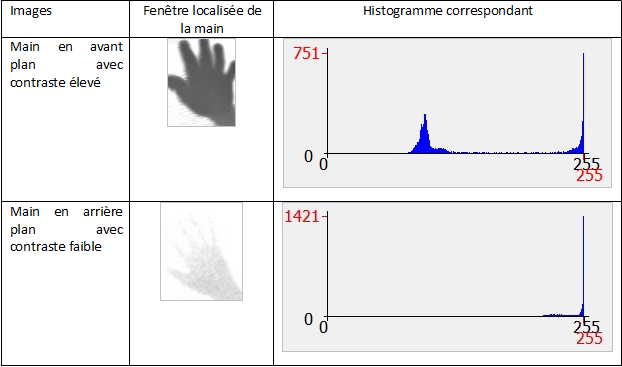
\includegraphics{table4.png}}
\caption{Histogrammes selon la luminosité et le contraste.}
\label{fig:histoLumin}
\end{figure}

Comme l’atteste le tableau ci-dessus (\autoref{fig:histoLumin}), nous avons affaire à des histogrammes bimodaux, même si c’est moins prononcé dans le second exemple de la main claire(en raison du nombre très élevé de valeurs de blanc). Il est cependant possible que l’histogramme ne suive pas le même schéma  et notamment que le deuxième mode ne soit pas 255 par exemple si on objet se trouve derrière la main ou si la main est devant le corps.
	La technique utilisée consiste à couper l’histogramme en deux parties via sa médiane (non pas sa moyenne). On recherche ensuite le mode sur le premier sous histogramme qui représente le niveau de gris le plus présent dans la main. On retient pour valeur de seuil un niveau de gris un peu plus élevé que le mode afin de seuiller la majeure partie de la main.

\[
Thresh = mode + n
\]
	Ca paramètre $n$ égal à 10 doit varier selon le contraste de la main. En effet, ce paramètre dépend de l’étendue de la première cloche de l’histogramme représentant le contraste de la main. Un faible contraste demandera une valeur faible tandis qu’un grand contraste demandera une valeur plus élevée. Tout l’enjeu ici est de seuiller correctement la main. Si le seuillage est trop faible ou trop élevé la binarisation donnera une image intraitable par le système de reconnaissance.